Nella periodo di Progettazione in dettaglio e codifica l'impengo in ore dei singoli componenti del gruppo non è stato omogeo: la presenza di uno studente lavoratore a tempo pieno, impegato all'interno del settore dei trasporti, ha rallentato le attività di sviluppo del prodotto. In particolare, sono stati altri componenti a farsi carico di alcune ore non svolte. Tale difformità si manifesta anche nelle conoscenze dei singoli individui all'interno del gruppo: le tecnologie che vengono apprese soprattutto durante le attività di codifica e di progettazione, svolte durante tutta la settimana dagli studenti, portano alla creazione di un gap di conoscenze che è difficile sanare se non si segue constantemente il progetto. Il \RdP{} ha provveduto a contattare i singoli membri del gruppo che sono risultati poco attivi ed a informare il gruppo sull'andamento della situazione. Nonostante tali difficoltà, SWEight intende consegnare il progetto e participare alla \RA{} a Maggio, per permettere ai componenti in regola con gli esami di laurearsi nella sessione di Luglio. Il \RdP{} provvede ad attuare le seguenti strategie al fine di ridurre i rischi riscontrati e permettere la consegna del prodotto alla proponente:
\begin{itemize}
	\item Le attività di codifica verranno marginalmente affidate allo studente lavoratore al fine di fornigli conoscenza sulle tecnologie impiegate e ridurre il rischio di iterazione;
	\item Le attività di maggior importanza vengono iniziate il weekend al fine di permettere a coloro che lavorano di partecipare in maniera attiva;
	\item Ripianificazione periodo destinato alle attività di verifica e validazione.
\end{itemize}
Malgrado le problematiche sopra esposte i singoli componenti sono consapevoli che la situazione non può avere ampi margini di miglioramento e l'armonia all'interno del gruppo è buona.\\
\begin{figure}[H]
\centering
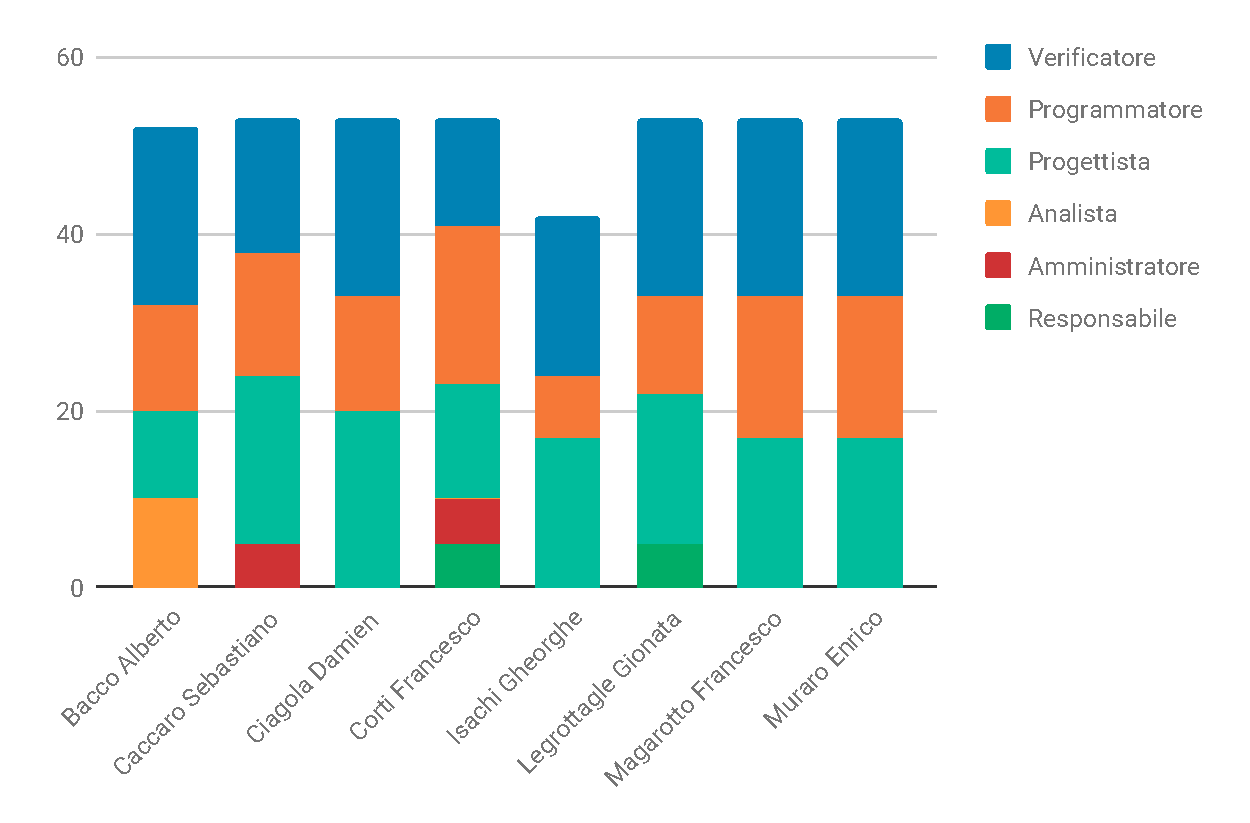
\includegraphics[scale=.8]{Consuntivo/grafici/ConsCod.pdf} 
\caption{Grafico orario per componente a fine periodo}
\end{figure}
\paragraph{Technology Baseline} \mbox{}\\
A seguito della \RP{} il gruppo ha provveduto a implementare una soluzione alternativa rispetto a quella proposta: il database Firestore è stato sostituito con MongoDB, alternativa open-source e pertanto priva di costi di licenza. Tale scelta è conseguente alla richiesta del docente Cardin di collegare il {database}\ped{G} alla backend al fine di ridurre l'accoppiamento. Lo studio di fattibilità di tale soluzione ha portato a complessità inaspettate, soprattutto nella stesura del codice Java, pertanto si è ritenuto provare ad implementare una nuova soluzione, dopo aver contattato e ottenuto l'approvazione da parte della proponente e dal docente Cardin. In relazione al fatto che entrambi i database sono documentali, pertanto la struttura delle collezioni è pressoché identica, e l'integrazione di Spring con MongoDB supportata dalla libreria Spring Data Mongo ha ridotto drasticamente la complessità del codice necessario. Pertanto, il cambio di tecnologia non ha portato a ritardi.